\documentclass[12pt, titlepage]{article}

\usepackage{booktabs}
\usepackage{tabularx}
\usepackage{hyperref}
\usepackage{graphicx}
\usepackage{float}
\graphicspath{ {./images/} }
\hypersetup{
    colorlinks,
    citecolor=black,
    filecolor=black,
    linkcolor=red,
    urlcolor=blue
}
\usepackage[round]{natbib}
\newcounter{NFR_Counter}
\addtocounter{NFR_Counter}{1}
\newcounter{FR_Counter}
\addtocounter{FR_Counter}{1}

\title{Software Requirements Specification\\\progname}

\author{\authname}

\date{}

%% Comments

\usepackage{color}

\newif\ifcomments\commentstrue %displays comments
%\newif\ifcomments\commentsfalse %so that comments do not display

\ifcomments
\newcommand{\authornote}[3]{\textcolor{#1}{[#3 ---#2]}}
\newcommand{\todo}[1]{\textcolor{red}{[TODO: #1]}}
\else
\newcommand{\authornote}[3]{}
\newcommand{\todo}[1]{}
\fi

\newcommand{\wss}[1]{\authornote{blue}{SS}{#1}} 
\newcommand{\plt}[1]{\authornote{magenta}{TPLT}{#1}} %For explanation of the template
\newcommand{\an}[1]{\authornote{cyan}{Author}{#1}}

%% Common Parts

\newcommand{\progname}{Software Engineering} % PUT YOUR PROGRAM NAME HERE
\newcommand{\authname}{Team 14, Reach
\\ Aamina Hussain
\\ David Moroniti
\\ Anika Peer
\\ Deep Raj
\\ Alan Scott} % AUTHOR NAMES                  

\usepackage{hyperref}
    \hypersetup{colorlinks=true, linkcolor=blue, citecolor=blue, filecolor=blue,
                urlcolor=blue, unicode=false}
    \urlstyle{same}
                                


\begin{document}

\maketitle

\pagenumbering{roman}
\tableofcontents
\listoftables
\listoffigures

\begin{table}[bp]
\caption{\bf Revision History}
\begin{tabularx}{\textwidth}{p{3cm}p{2cm}X}
\toprule {\bf Date} & {\bf Version} & {\bf Notes}\\
\midrule
Date 1 & 1.0 & Notes\\
Date 2 & 1.1 & Notes\\
\bottomrule
\end{tabularx}
\end{table}

\newpage

\pagenumbering{arabic}

This document describes the requirements for the web application REACH. The template for the Software
Requirements Specification (SRS) is a subset of the Volere
template~\citep{RobertsonAndRobertson2012}.  If you make further modifications
to the template, you should explicitly state what modifications were made.

\section{Project Drivers}

\subsection{The Purpose of the Project}

The purpose of this project is to create a web application, REACH, which will help people find and apply to clinical trials that they are eligible for. Currently there is no intuitive path between researchers and patients which patients can use to apply to a clinical trial. Existing databases of these clinical trials are often hard to navigate, especially for those who do not have experience with medical terminology. The completed application will allow users to find clinical trials for which they may be eligible, and give users a method of contacting the research coordinator for that trial.

\subsection{The Stakeholders}

\subsubsection{The Clients}

The clients for this project are our project supervisors: Dr. Terrence Ho, and Dr. Cieran Scallan. 

\subsubsection{The Customers}

The customers for this project are people who are looking to take part in a clinical trial.

\subsubsection{Other Stakeholders}

Other stakeholders for this project are researchers who will be contacted by patients using this application.

\subsection{Mandated Constraints}

The constraints for this project are:

\subsubsection{Implementation Constraints}
The project must be accessible from the web with the need for installation of any applications other than a web browser.

\subsubsection{Schedule Constraints}
The project must be completed within the 8 month period of the school year.

\subsubsection{Budget Constraints}
The project must not use more than \$750.

\subsection{Naming Conventions and Terminology}

\begin{itemize}
    \item Platform - The web system/application.
    \item Heavy traffic - When many users are accessing the platform at one time.
    \item NIST - National Institute of Standards and Technology
    \item Patient - An individual with a given medical condition(s) who is seeking to enroll in medical research studies.
    \item Clinician - A medical care provider enrolling a patient in research studies on their behalf.
    \item Organizer - Person or organization seeking patients for their research study.
\end{itemize}

\subsection{Relevant Facts and Assumptions}

It is assumed that users of the application will vary in age, ability, and how much experience they have in using web applications. 

\section{Functional Requirements}

\subsection{The Scope of the Work and the Product}

\subsubsection{The Context of the Work}

\subsubsection{Work Partitioning}

\subsubsection{Individual Product Use Cases}

\begin{enumerate}

\item \textit{Patient Account Creation}. A patient creates an account to store their clinical data. The user first selects to create an account. They provide a username and password, along with their email. Once this is verfied, they input their information (weight, height, birthday, medical conditions, address). Upon entering valid inputs, the user is informed that their account is created and they are logged in.

\item \textit{Patient Login}. A patient logs into their account. When a patient clicks the login button, they are presented with the login menu. Once they input their credentials and login, the system verifies that their details are valid and logs them in. If not, the user is informed of the incorrect credentials and is prompted to try again.

\item \textit{Input Search Parameters}. The user inputs search parameters into the search fields to filter available studies. This use case is optional as a logged in user will automatically search by their saved paraters.

\item \textit{Search for Studies}. Using input parameters, studies are retrieved from the repository, filtered, and displayed to the user. 

\item \textit{Send Email to Organizer}. Once a patient selects a study, they can use the application to send an email to the organizer of the study.

\item \textit{Patient Profile Modification}. A patient modifies their profile to change certain attributes (weight, height, birthday, medical conditions, address). The patient selects the UI element that opens their profile and modifies the respective fields. They save and the server updates their information on the database. 

\begin{figure}[H]
\centering
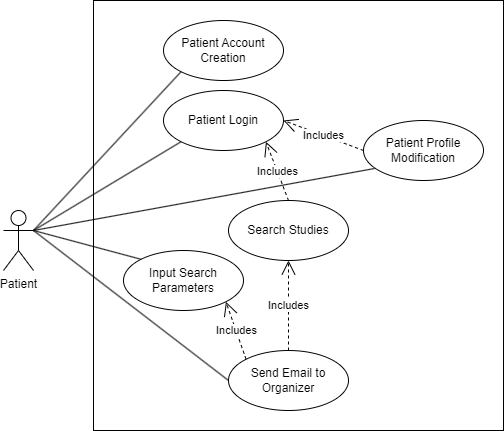
\includegraphics[scale=0.5]{PatientUseCase.png}
\caption{Patient use case diagram}
\end{figure}

\end{enumerate}

\subsection{Functional Requirements}

\textbf{FR-\the\value{FR_Counter}:}
The system shall enable the user to create an account before signing in to the application. Account credentials must include 
an email and a password satisfying the NIST password guidelines.\\
\textbf{Rationale:}
Many application features will be reliant on a user account/email. Additionally, to ensure the safety/security of sensitive information,
it is important to enforce strict password guidelines. \\
\textbf{Fit criterion:}
The system shall log the user in to their newly created account upon successful creation. \\~\\
\addtocounter{FR_Counter}{1}

\noindent{\textbf{FR-\the\value{FR_Counter}:}}
The system shall ensure the same email cannot be used across multiple accounts.\\
\textbf{Rationale:}
The email needs to be a unique identifier of an account.\\
\textbf{Fit criterion:}
The system shall inform a user if the email they entered is already in use under another account. \\~\\
\addtocounter{FR_Counter}{1}

\noindent{\textbf{FR-\the\value{FR_Counter}:}}
The system shall enable a user to sign in to an existing account.\\
\textbf{Rationale:}
To use all of the application features a user must be signed in to their account.\\
\textbf{Fit criterion:}
The system shall log the user into the application upon validation of the credentials they entered. If invalid credentials are entered,
the user should be informed of this error. \\~\\
\addtocounter{FR_Counter}{1}


\noindent{\textbf{FR-\the\value{FR_Counter}:}}
The system shall enable a user to sign in to the application as a guest.\\
\textbf{Rationale:}
Some features of the application do not require a full account, so the user should have the option to sign in as a guest
if they only require a subset of the application's features.\\
\textbf{Fit criterion:}
The system shall log the user into the application as a guest upon entering an identifier for the current session. \\~\\
\addtocounter{FR_Counter}{1}


\noindent{\textbf{FR-\the\value{FR_Counter}:}}
The system shall enable a user to reset their password before signing in to the application.\\
\textbf{Rationale:}
It is likely some users will forget their password, and will need to reset it to be able to log back into their account.\\
\textbf{Fit criterion:}
The system shall send the user an email (to the email tied to the account they are trying to log into), allowing them to 
create a new password. The user should be logged into their account upon entering a new, valid password.\\~\\
\addtocounter{FR_Counter}{1}


\noindent{\textbf{FR-\the\value{FR_Counter}:}}
The system shall enable a user to sign out of the application.\\
\textbf{Rationale:}
Users should be able to sign out for both security reasons, and practical reasons.\\
\textbf{Fit criterion:}
The system shall return the user to the main landing page upon signing out of their account.\\~\\
\addtocounter{FR_Counter}{1}


\noindent{\textbf{State machine for user login/signup:}}
\begin{itemize}
    \item Precondition - User is on the initial page of the app
    \item Postcondition - User is logged in to application
    \item Intermediary States:
    \begin{itemize}
        \item User is in the process of signing in
        \item User is in the process of creating an account
        \item User is in the process of resetting their password
    \end{itemize} 
\end{itemize}

\begin{figure}[H]
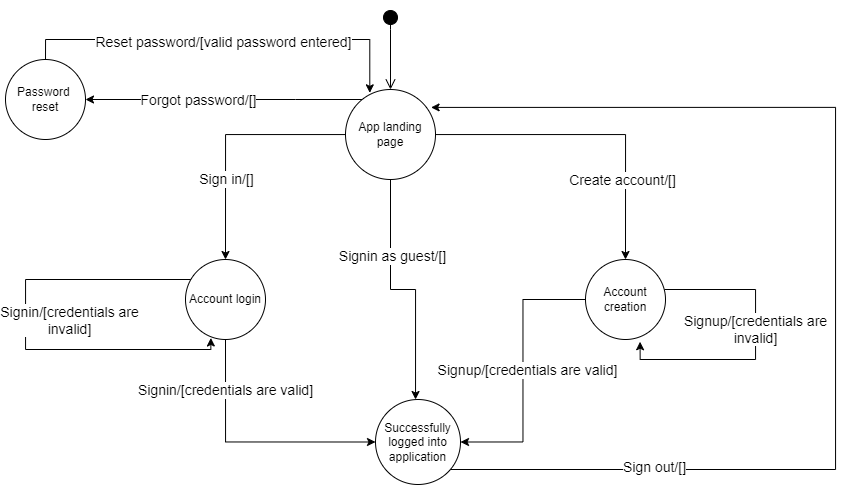
\includegraphics[width=\textwidth]{Signup_state_machine}
\end{figure}


\noindent{\textbf{FR-\the\value{FR_Counter}:}}
The system shall prompt a user to enter information about themselves and their medical history 
upon creation of an account (i.e., first time signing on), or when a user signs on as a guest.\\
\textbf{Rationale:}
The system must know information about the user to match them to potential clinical trials.\\
\textbf{Fit criterion:}
After a user signs on for the first time, they should be asked to enter their date of birth, height, weight, gender, and 
current address. Additionally, they should be asked to enter any medications they take, and any medical conditions that they have.\\~\\
\addtocounter{FR_Counter}{1}

\noindent{\textbf{FR-\the\value{FR_Counter}:}}
The system shall store the information entered by a user with an account in the database.\\
\textbf{Rationale:}
The system shall only need to ask users with an account for their information once.\\
\textbf{Fit criterion:}
The system shall be able to retrieve the information tied to a users account after they have signed out of the application. \\~\\
\addtocounter{FR_Counter}{1}


\noindent{\textbf{FR-\the\value{FR_Counter}:}}
The system shall enable a user to update the personal information tied to their account.\\
\textbf{Rationale:}
Personal characteristics and circumstances are always changing, and a user should be able to make these changes in the application.\\
\textbf{Fit criterion:}
The updates made by the user shall be reflected in both the UI (for the user to see) and in the database.\\~\\
\addtocounter{FR_Counter}{1}

\noindent{\textbf{FR-\the\value{FR_Counter}:}}
The system shall create an email template for the user to send their interest in participating in a trial to the research coordinator.\\
\textbf{Rationale:}
Users may not know what they need to include in the email, so the template should simplify this process.\\
\textbf{Fit criterion:}
The system shall output an email template. The email template shall include all relevant information that the user has provided and details about the trial they wish to participate in.\\~\\
\addtocounter{FR_Counter}{1}

\noindent{\textbf{FR-\the\value{FR_Counter}:}}
The system shall notify the user when new medical trials matching their specifications are available, if requested by the user.\\
\textbf{Rationale:}
New medical trials matching the users specifications which the user may want to participate in may be started after the user searches initially, this feature means the user would not have to search every couple of days for new trials.\\
\textbf{Fit criterion:}
The system shall notify the user about new trials with parameters that they specified.\\~\\
\addtocounter{FR_Counter}{1}

\noindent{\textbf{FR-\the\value{FR_Counter}:}}
The system shall include frequently asked questions and information about how medical trials work.\\
\textbf{Rationale:}
Users may not be aware of how medical trials work exactly, and this may cause confusion for the user when searching for a medical trial.\\
\textbf{Fit criterion:}
The system shall contain and display information about medical trials, and answers to questions the users may commonly have.\\~\\
\addtocounter{FR_Counter}{1}

\section{Non-functional Requirements}

\subsection{Look and Feel Requirements}

\subsection{Usability and Humanity Requirements}

\textbf{NFR-\the\value{NFR_Counter}:}
The application interface shall be intuitive to use to a point where users do not require a tutorial or help from another person. \\
\textbf{Rationale:}
The interface will be used by users with a wide range of technical ability, so making the interface as easy to learn as possible will make the application maximally accessible. \\
\textbf{Fit criterion:}
95\% of users tested should be able to accomplish the main function of the application without need for outside intervention. \\
\textbf{Traceability:}
Traces to functional requirements involving the user interface. \\~\\
\addtocounter{NFR_Counter}{1}

\noindent\textbf{NFR-\the\value{NFR_Counter}:}
The application interface shall only include the minimum necessary elements for the system to function effectively. \\
\textbf{Rationale:}
The simplicity of the system is important to ensure that the system is easy for all users to interact with. \\
\textbf{Fit criterion:}
Testers should not be able to identify any element of the user interface that does not serve any immediate and apparent use. \\
\textbf{Traceability:}
Traces to functional requirements involving the user interface. \\~\\
\addtocounter{NFR_Counter}{1}

\noindent{\textbf{NFR-\the\value{NFR_Counter}:}}
The text and image elements of the user interface should be large enough such that  \\
\textbf{Rationale:}
Due to the nature of the system, it can be expected that users of varying visual aptitude will be interacting with the user interface. Making the interface visually accessible will ensure that users of non-perfect optical perscriptions are not excluded from its use. \\
\textbf{Fit criterion:}
A user with a prescription of less than 4 diopters should be able to effectively use the interface without the use of perscription glasses. Alternatively, a perfectly sighted individual should be able to read the interface 1 meter away from their computer monitor without issue. \\
\textbf{Traceability:}
 \\~\\
\addtocounter{NFR_Counter}{1}


\subsection{Performance Requirements}

\textbf{NFR-\the\value{NFR_Counter}:}
The system shall load and display trials to the user in a timely manner.\\
\textbf{Rationale:}
In addition to obvious usability reasons, there is a potential for users (especially clinicians) to rapidly
change the criteria for eligibility, meaning the time spent waiting for trials to load can grow very fast if it is slow.\\
\textbf{Fit criterion:}
The system shall not take longer than 5 seconds to load and display a set of trials, during any given search made by a user.\\
\textbf{Traceability:}
**Traces to functional requirements related to searching for trials, displaying trials, getting data from repositories.** \\~\\
\addtocounter{NFR_Counter}{1}

\noindent{\textbf{NFR-\the\value{NFR_Counter}:}}
The system shall remain performant during times of heavy traffic.\\
\textbf{Rationale:}
The system will experience varying amounts of traffic, and it should be prepared to handle all cases (heavy traffic being the 
one to likely cause issues).\\
\textbf{Fit criterion:}
Any system API call shall take less than 1 second to respond for up to 1000 concurrent users, and less than 2 seconds to respond for anything 
greater (assuming the system will not see $>10000$ users).\\
\textbf{Traceability:}
Traces to pretty much all FRs that are mentioned in the other performance requirements \\~\\
\addtocounter{NFR_Counter}{1}

\noindent{\textbf{NFR-\the\value{NFR_Counter}:}}
The systems UI elements shall acknowledge all forms of user input in a timely manner.\\
\textbf{Rationale:}
Timely response from the system is necessary for a good user experience. Additionally, things like keyboard
shortcuts should be just as performant as using a mouse (and vice-versa).\\
\textbf{Fit criterion:}
The system shall take less than 150ms to acknowledge user input, and make it clear to the user that it has registered the request.\\
\textbf{Traceability:}
Traces to any FR that requires user input of some form \\~\\
\addtocounter{NFR_Counter}{1}

\noindent{\textbf{NFR-\the\value{NFR_Counter}:}}
The system shall efficiently store/retrieve user data from the database.\\
\textbf{Rationale:}
For the system to remain performant, it must handle data efficiently, especially as the total number of users increase.\\
\textbf{Fit criterion:}
The system shall take no longer than 500ms when querying the database for user info (includes query execution time + any overhead of executing 
the query).\\
\textbf{Traceability:}
Traces to any FR that requires user information \\~\\
\addtocounter{NFR_Counter}{1}

\noindent{\textbf{NFR-\the\value{NFR_Counter}:}}
The system shall be available to users 99\% of the time.\\
\textbf{Rationale:}
Since users will likely make infrequent visits to the platform, it is necessary that the platform will be available at those 
times (i.e., if the system is frequently unavailable, it increases the chances that users will never use the platform).\\
\textbf{Fit criterion:}
The system shall experience no more than 15 hours of downtime throughout the year.\\
\textbf{Traceability:}
N/A
\addtocounter{NFR_Counter}{1}

\subsection{Operational and Environmental Requirements}

\noindent{\textbf{NFR-\the\value{NFR_Counter}:}}
The system shall interface with data from ClinicalTrials.gov and/or some other medical trials repositories.\\
\textbf{Rationale:}
The system needs to gather trials from a preexisting data source so that it can match patients to them.\\
\textbf{Fit criterion:}
The system should have a similar number(within order of magnitude) of currently running clinical trials as ClinicalTrials.gov for users to search from.\\
\textbf{Traceability:}
Any FRs which retrieve data from a data source \\~\\
\addtocounter{NFR_Counter}{1}

\noindent{\textbf{NFR-\the\value{NFR_Counter}:}}
The system shall be able to be used on any most modern devices which are capable of browsing the web.\\
\textbf{Rationale:}
Users will likely use a large variety of devices from phones to PCs, so it is necessary to support them, (i.e. users are less likely to use the application if it doesn't work on mobile).\\
\textbf{Fit criterion:}
The system shall work on at least 80\% of devices which have web browsers and were released in the last 5 years.\\
\textbf{Traceability:}
N/A \\~\\
\addtocounter{NFR_Counter}{1}

\subsection{Maintainability and Support Requirements}


\noindent{\textbf{NFR-\the\value{NFR_Counter}:}}
The system shall be easy to fix in the event it experiences unexpected downtime.\\
\textbf{Rationale:}
While it may not happen often, an unexpected system failure is definitely possible. As the time it takes 
to fix the issue increases, so does the number of users negatively affected.\\
\textbf{Fit criterion:}
On average, it should take less than 1 hour to restore the system in the event of a failure.\\
\textbf{Traceability:}
N/A \\~\\
\addtocounter{NFR_Counter}{1}


\noindent{\textbf{NFR-\the\value{NFR_Counter}:}}
The system shall be adaptable to new requirements.\\
\textbf{Rationale:}
It is likely new requirements will be discovered once users begin to use the platform, and there will be a need/desire to 
implement these quickly and effectively.\\
\textbf{Fit criterion:}
The system must satisfy all of its existing requirements after the implementation of a new requirement/feature.\\
\textbf{Traceability:}
N/A
\addtocounter{NFR_Counter}{1}


\subsection{Security Requirements}
\noindent\textbf{NFR-\the\value{NFR_Counter}:}
test
\addtocounter{NFR_Counter}{1}

\subsection{Cultural Requirements}
\noindent\textbf{NFR-\the\value{NFR_Counter}:}
The interface shall be useable by users who speak a language other than English or French.  \\
\textbf{Rationale:}
Restricting the interface's language to only official languages will exclude many ethnic minorities from being able to access clinical studies. Making the program multilingual will ensure that a minimal number of ethnic minorities will be excluded. \\
\textbf{Fit criterion:}
Users who speak the languages in the top 5 most spoken non-official languages in Canada should be able to use the interface without issue. \\
\textbf{Traceability:}
Traces to functional requirements involving the user interface. \\~\\
\addtocounter{NFR_Counter}{1}

\subsection{Legal Requirements}
\noindent\textbf{NFR-\the\value{NFR_Counter}:}
The system shall conform to regulations regarding the collection, storage, and usage of medical information.  \\
\textbf{Rationale:}
Since the data stored pertains to personal medical information, we are legally required to manage the data in such a way that protects the personal information of the patients. \\
\textbf{Fit criterion:}
The system should be able to pass an independent audit to ensure the data is being collected and secured in an appropriate manner. \\
\textbf{Traceability:}
Traces to requirements involving user input (specifically medical data input) and security requirements. \\~\\
\addtocounter{NFR_Counter}{1}

\subsection{Health and Safety Requirements}

This section is not in the original Volere template, but health and safety are
issues that should be considered for every engineering project.

\section{Project Issues}

\subsection{Open Issues}

\subsection{Off-the-Shelf Solutions}

\subsection{New Problems}

\subsection{Tasks}

\subsection{Migration to the New Product}

\subsection{Risks}

\subsection{Costs}

\subsection{User Documentation and Training}

\subsection{Waiting Room}

N/A

\subsection{Ideas for Solutions}

\subsection{Anticipated Changes}

Below are some changes that could potentially be made to future 
revisions of the SRS for this application, depending on several factors,
such as unexpected costs/issues arising during development (or even the lack 
of expected costs/issues during development).

\begin{itemize}
    \item Two different types of accounts - one for patients and one for clinicians
    \item Clinician account specifically designed for finding clinical trials on behalf of patients
    \item Clinician account enables saving patient's information (i.e., clinicians can have their own personal database of patients)
    \item The types of information collected should be expected to change frequently, especially as development begins and users begin testing the application
\end{itemize}

\bibliographystyle{plainnat}

\bibliography{SRS}

\newpage

\section{Appendix}

N/A

\subsection{Symbolic Parameters}

N/A


\end{document}